Digamos que tenemos un árbol y queremos calcular para cada nodo del árbol la longitud máxima de un camino que comienza en ese nodo. Esto puede verse como una generalización del problema del diámetro del árbol, porque la mayor de esas longitudes es igual al diámetro del árbol. 

Como ejemplo, considere el siguiente árbol:

% TODO: \usepackage{graphicx} required
\begin{figure}[h!]
	\centering
	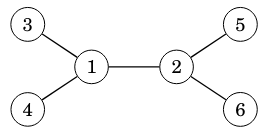
\includegraphics[width=0.4\linewidth]{img/all_longest_paths_1}

	\label{fig:alllongestpaths1}
\end{figure}

Sea $maxLength(x)$ la longitud máxima de una ruta que comienza en el nodo $x$. Por ejemplo, en el árbol anterior, $maxLength(4) = 3$, porque hay una ruta $4 \rightarrow 1 \rightarrow 2 \rightarrow 6$. Aquí hay una tabla completa de los valores:

$$
\begin{array}{r|cccccc}
\text{node x} 	& 1 & 2 & 3 & 4 & 5 & 6 \\
maxLength(x) 	& 2 & 2 & 3 & 3 & 3 & 3
\end{array}
$$

En la presente guía abordaremos como determinar para cada nodo del árbol la longitud máxima de un camino que comienza en ese nodo